\documentclass{article}
\usepackage{mathtools}
\usepackage{tikz}
\usepackage{pgfplots}
\usepackage{bm}
\usepackage{graphicx}
\usepackage{fancyhdr}
\usepackage{indentfirst}
\usepackage{titlesec}
\usepackage{multicol}
\usepackage{listings}
\usepackage{graphicx}
\usepackage{tabularx}
\usepackage{amsfonts}
\usepackage{placeins}
\usepackage{titlesec}
\usepackage{algorithm}
\usepackage{pst-electricfield}
\usepackage[noend]{algpseudocode}
\usepackage{textcomp}
\usepackage{sidecap}
\usepackage[
backend=biber,
style=alphabetic,
sorting=ynt
]{biblatex}
\addbibresource{sources.bib}
\usepackage{color} %red, green, blue, yellow, cyan, magenta, black, white
\definecolor{mygreen}{RGB}{28,172,0} % color values Red, Green, Blue
\definecolor{mylilas}{RGB}{170,55,241}

\lstset{language=Matlab,%
    %basicstyle=\color{red},
    breaklines=true,%
    morekeywords={matlab2tikz},
    keywordstyle=\color{blue},%
    morekeywords=[2]{1}, keywordstyle=[2]{\color{black}},
    identifierstyle=\color{black},%
    stringstyle=\color{mylilas},
    commentstyle=\color{mygreen},%
    showstringspaces=false,%without this there will be a symbol in the places where there is a space
    numbers=left,%
    numberstyle={\tiny \color{black}},% size of the numbers
    numbersep=9pt, % this defines how far the numbers are from the text
    emph=[1]{for,end,break},emphstyle=[1]\color{red}, %some words to emphasise
    %emph=[2]{word1,word2}, emphstyle=[2]{style},    
}

\sidecaptionvpos{figure}{c}

\setlength{\columnsep}{1cm}

\setcounter{secnumdepth}{4}

\titleformat{\paragraph}
{\normalfont\normalsize\bfseries}{\theparagraph}{1em}{}
\titlespacing*{\paragraph}
{0pt}{3.25ex plus 1ex minus .2ex}{1.5ex plus .2ex}


\pagestyle{fancy} % Default page style 
\lhead{Nic Fishman}
\chead{}
\rhead{\thepage}
\lfoot{}
\cfoot{}
\rfoot{}


\titlelabel{\thetitle\enspace}

\begin{document}

\title{%
  Fleeing from Terror \\
  \large Considering Safety When Designing Public Spaces \\
  in the Age of Radicalization}
\author{Nic Fishman}
\maketitle

\abstract{
Sometimes, the safest thing people can do is flee from danger. But what if they're in a room with dozens, or hundreds, of other people when that danger arises? How do they get out? And did the people who designed the room they are in, whether it's an intimate theater or a concert hall or a sprawling convention center, think about how to get people out the doors --- fast --- in an emergency?

In the following paper we outline a methodology for evaluating a room on the basis of safety, taking the time for the room to evacuate in the case of a sudden terrifying event as our metric of safety. We also develop a way to optimize the design of a room for safety, and propose a regulatory framework for ensuring new construction is safe.}

\section{Introduction}

It is rare today in the United States that a theater catches fire and hundreds of people die. One hundred years ago, that particular tragedy was all too common, but decades of legislation, updated fire codes and improved building materials, have largely put a stop to theater fires.

Today, we face a tragedy of similar scale: mass shootings, motivated by radicalized individuals, who can do extraordinary damage. These shootings have increases in frequency and severity in recent years \cite{chalabi_2017}, and as the problem worsens, it becomes more and more clear that we need a policy solution. We need to keep people safe.

The most obvious answer would be gun control, but this is a highly contentious issue in the United States, in a way it has not proved anywhere else in the world. The next obvious place might be mental health screening, trying to catch people who are likely to commit these atrocities early, and stop them before they can hurt anyone. This seems logical, but experts have concluded "the sorts of individuals who commit mass murder often are either not mentally ill or do not recognize themselves as such. Because they blame the outside world for their problems, mass murderers would likely resist therapies that ask them to look inside themselves or to change their behavior." \cite{khazan_2017}

So if the two most obvious solutions don't seem viable, where should policy makers turn to make progress on this issue? They should look to the past; they should remember how the United States dealt with the issue of urban building fires; they should look to building codes.

There are a lot of types of public spaces that have become targets in recent years --- theaters, schools, churches, malls, arenas. These spaces are all designed with various criteria in mind, but none of them are designed taking into consideration how people could flee in the case of an attack. In the following paper, we propose an objective framework for evaluating a theater's ``Time to Exit" (I use the word ``theater" as a stand-in for all kinds of similar places where people gather, from convention centers to stadiums to movie theaters to classrooms). This ``Time to Exit" (TTE) is the amount of time it would take everyone to evacuate in the case of an attack. If we can also somehow derive a TTE for the optimal design of a given theater, then we can evaluate how safe a theater is, as compared to how safe it could be. This framework can then be applied in a regulatory setting, allowing legislating bodies to set an acceptable threshold on how far from optimal a theater's TTE can be, and evaluating new construction based on this metric.

While we figure out how to stop the attacks themselves, we can at least give people out enjoying themselves the best possible chance of getting to safety. This analysis --- the algorithm we've developed --- is one step in that direction.

\section{Modeling Crowd Dynamics}

The objective here is relatively straightforward: given the set up of a theater, its dimensions, location of obstacles, location of exits, the initial position of the people in the theater, and the position of the terror (this is whatever thing or person people are afraid of; it can be an actual terrorist, a fire, an explosion --- anything people would be repulsed from), how long does it take everyone to get out of the theater?

\subsection{The Metropolis Method}

Human behavior is notoriously multifaceted and difficult to predict, so to make the problem more approachable we need a model; some system that will represent the more complicated crowd dynamics problem, preferably in a less computationally intensive way. It is at this point that we turn to chemistry.

A common problem in molecular simulation is fluid dynamics: how can we simulate the behavior of liquids, at various temperatures, pressures, in various volumes. The issue is that if the program has to account for all of the forces between all of the particles at each time step, then the program will be incredibly computationally inefficient, especially for large numbers of particles. The solution to this issue is called ``Hard Sphere Simulation", where every molecule is assumed to be a sphere (or, in two dimensions, a circle), and all spheres are considered ``hard", in that they are not allowed to overlap. Spheres are assumed to have no interaction unless they're overlapping, in which case they have infinite potential. 

This is a rather interesting solution, but it creates a huge problem: how should the velocity of the particles be accounted for if there is no force calculation? How do chemists move the particles to new positions at each iteration of the simulation? This seems rather daunting, but there is a hero on the horizon -- probability. What chemists do is randomly permute all the particles via some symmetrical distribution on every axis. We will call this a move. This is of course not a complete solution to the problem. Because chemists want their simulation to accurately simulate reality, they cannot just randomly move the particles and be done, they have to decide whether the move was ``good": that is whether it was accurate to reality. Chemists use a special function, called an acceptance criterion, to decide whether to accept a move. The acceptance criterion is actually the probability that the system moves from the old state $o$ to the new state $n$. This can be calculated using a distribution called the Maxwell-Boltzmann distribution, which takes a change in potential energy for a system, and returns a probability of that change:

\begin{equation}
	x \sim Uni(0,1)
\end{equation}

\begin{equation}
	acc(o \rightarrow n) = e^{-\frac{U(n) - U(o)}{kT}} > x
\end{equation}

So the acceptance criterion is a Bernoulli random variable that will accept a new state $n$, with potential energy $U(n)$, according to the PDF of the Maxwell-Boltzmann distribution, at temperature $T$ (the temperature is actually multiplied by the Boltzmann constant $k$, and in this paper this will be treated as one parameter $kT$). Then there is the random uniform variable; this is what makes the simulation true to reality. Anything is possible in a quantum mechanical world, some outcomes are just more likely. This acceptance criterion is designed to capture that fundamental truth about the randomness of quantum systems.

Combining all these components, the Metropolis algorithm is born \cite{frenkel_2001}:

\begin{algorithm}
\caption{This simple set of algorithms gives a high level appreciation for how simple the Metropolis algorithm can be. All that happens is $X$, the initial position of the particles, is moved $n$ times, each particle in $X$ given a random displacement according to a normal distribution with $\mu=0$ and $\sigma=\sigma_x$. A move is accepted if the particles do not overlap, otherwise it is rejected.}\label{metropilis}
\begin{algorithmic}[1]
\Procedure{metropolis}{$n$, $X$, $kT$, $\sigma_x$}
\State $U \gets \infty$
\For {i=1:n}
	\State $X, U \gets move(X, en, kT, \sigma_x)$
\EndFor
\State \textbf{return} $X, U$
\EndProcedure

\Procedure{move}{$X$, $en$, $kT$, $\sigma_x$}
\State $X_n \gets normrnd(\mu=0,\sigma=\sigma_x,n=len(X))$
\State $U_n \gets energy(X)$
\If{$exp(-(U_n - U) / kT) > rand$}
\State \textbf{return} $X_n, U_n$
\EndIf
\State \textbf{return} $X, U$
\EndProcedure

\Procedure{energy}{$X$}
\For{$x_i$ in $X$}
\For{$x_j$ in $X$}
\If{$overlap(x_i, x_j)$}
\State \textbf{return} $\infty$
\EndIf
\EndFor
\EndFor
\State \textbf{return} $0$
\EndProcedure
\end{algorithmic}
\end{algorithm}

\subsection{Extending to the Human Case}

How do we connect the movement of particles in a flowing liquid to people in a movie theater? The key insight is this: humans are like particles. As anyone who has ever left a stadium or arena knows, a group of people flows --- and hangs up --- much like a liquid. So this same type of Metropolis simulation can be used to at least approximate the randomness in human behavior, and it will do so very efficiently. This analogy also results in some interesting analogs. The $kT$ value can be thought of as the level of panic in the theater. How likely are people to be confused and go the wrong way? The $sigma_x$ value is the time proxy, the larger it is, the larger it is, the closer the simulation is to real time.

There is of course a major flaw: in the model as described so far, there is no motivating force. People would simply mill about in the theater, which will not fulfill the goal of the simulation. So how to motivate the ``particles" to move to the exit of the theater, while avoiding the terror?

Here the Metropolis analogy is once again useful. What if all the particles in the theater are negatively charged? The charge is negligible for particle-particle interactions, but the particles potential energy will be effected by an electric field. This is precisely the model needed to get the people in the simulation to move towards the exit: the exit will be simulated by a positive point charge, the terror by a negative point charge, and thus the people, which are negatively charged, will have lower potential the closer they are to the exit, and the further they are from the terror. This effect is shown in Figure 1: a negatively charge particle will be at lowest potential when it is closest to the positively charged particle.

\begin{figure}
\centering
\begin{pspicture*}(-5,-5)(5,5)
\psframe*[linecolor=white](-5,-5)(5,5)
\psgrid[subgriddiv=0,gridcolor=lightgray,griddots=10]
\psElectricfield[Q={[1 -2 0][-1 2 0]},linecolor=red]
\psEquipotential[Q={[1 -2 0][-1 2 0]},linecolor=blue](-5,-5)(5,5)
\psEquipotential[Q={[1 -2 0][-1 2 0]},linecolor=black,Vmin=0,Vmax=0](-5,-5)(5,5)
\end{pspicture*}
\caption{This shows the electric field created between two point charges. This will form the core of the model used to simulate the crowd dynamics problem at the heart of this paper.}
\end{figure}


This requires some minimal modification to the algorithms above, namely the energy function will now perform the following calculation, if $e$ is the vector position of the exit and $t$ the vector position of the terror:

\begin{equation}
	U = \sum_{x=X} \frac{kQ_t}{||x-t||} - \frac{kQ_e}{||x-e||}
\end{equation}

With this substitution, the Maxwell-Boltzmann acceptance criterion will over time force the simulation to it's lowest potential equilibria; the people will leave the theater.

Of course thus far the people have been moving about in an empty theater with one terror and one exit. To make this more realistic, the model needs to account for the theater containing some barriers, seats, railings, walls, columns, that people cannot easily pass through. For the model to account for this, it will accept some set of line segments and polygons that people cannot overlap with, in a similar way to how people cannot overlap with each other. This allows for the effective simulation of just about any theater using the model. 

\subsection{Extending to Multiple Exits}

There is one last issue with the model up to this point. It only allows for a theater to have one exit. If we added a second or a third exit, there would be an optimal point in between the two exits, where moving in either direction would cause an increase in potential that the acceptance criterion is unlikely to accept. The system would likely achieve a steady state equilibrium without everyone evacuating the theater. Some people will just be paralyzed between the two exits.

The simplest, most efficient solution to this problem is to say that people are ``smart." They will know what exit is closest to them, and only experience the attractive force of that exit. This greatly simplifies the calculation for multiple exits, and elegantly solves the equilibria problem.

All that needs to be changed to incorporate these adaptations of the model is the energy function. See the modified energy function in Algorithm 2.

\begin{algorithm}
\caption{This iteration of the energy algorithm takes $X$, the current position of the people, $B$, the position of all barriers, $E$ the position of all exits, $t$, the position of the terror, and $l$ and $w$, the dimensions of the theater. The overlap functions are in reality specific to the shapes being compared and involve a bit of interesting geometry, but have been excluded here for succinctness.}\label{basic_energy}
\begin{algorithmic}[1]
\Procedure{energy}{$X$, $B$, $E$, $t$, $l$, $w$}

\State $\triangleright$ Check if any people are out of the bounds of the simulation
\If{$any\_out\_of\_bounds(X, l, w)$}
\State \textbf{return} $\infty$
\EndIf

\For {$i \gets 1:len(X)$}

\State $\triangleright$ Check if person overlaps any barriers
\If{$any\_overlap(X(i), B)$}
\State \textbf{return} $\infty$
\EndIf

\State $\triangleright$ Check if person overlaps any people
\If{$any\_overlap(X(i), X(i+1:end))$}
\State \textbf{return} $\infty$
\EndIf
\EndFor

\State $U_n \gets 0$

\For {$x$ in $X$}
\State $\triangleright$ Get closest exit, do potential calculation, and add to summation
\State $e \gets get\_closest\_exit(x, E)$
\State $U_n \gets U_n + \frac{1}{||x-t||} - \frac{1}{||x-e||}$
\EndFor
\State \textbf{return} $U_n$

\EndProcedure
\end{algorithmic}
\end{algorithm}

\subsection{Summary}

The way core of the framework that is the subject of this paper is the ability to simulate the way people would flee a tehater with a terrifying actor at some point in the theater. To do this simulation, the framework takes inspiration from chemistry, using a heavily modified version of the Metropolis algorithm that chemists use to simulate fluid dynamics. This is actually a Monte Carlo algorithm --- a randomized algorithm whose output is a random variable. The framework will model TTE for any size theater, with any number of people, with any number of barriers in the theater. 

\section{Runtime Optimization}

Even though this algorithm is fast, it has some issues that can cause really long runtimes. At this point the algorithm runs in about 13 seconds for the test theater, which is a longer runtime than would be optimal. The algorithm is $O(||X||^2)$ for the number of people in the theater, as the energy calculation checks whether all people are overlapping with all other people. This section introduces some techniques used to improve both of these issues, making the framework faster and more scaleable.

\subsection{Cell Lists}

To fix the scalability issues, the framework can borrow an idea from another area of chemistry. Sometimes chemists don't want a probabilistic analysis of a chemical system, but are looking for a true to life simulation. When they want to do a simulation that is governed by classical mechanics, where all the particles are moving according to Maxwell's equations for electric force, that is called molecular dynamics. Molecular dynamics has to deal with the same issues as noted in Section 2.2: namely that calculating the forces between all the particles in the system is incredibly computationally intensive. This lead to the development of a technique known as cell lists.\cite{allen_1989}

\begin{SCfigure}
    \includegraphics[width=0.25\textwidth]{celllist.png}
    \caption{(a) This diagram is what molecular dynamics seeks to simulate; the interaction between the particle of interest and all other particles. (b) This shows what cell lists simulate, the interaction between the particle of interest, all particles in the same cell, and all particles in neighboring cells. \cite{wikipedia_2016}}
\end{SCfigure}

Cell lists are a way of breaking up the simulated space into equally sized blocks, and then only computing interactions between particles in adjacent cells. This means that especially for simulations with many particles, the number of required calculations is much lower (see Figure 2). The framework can make use of this idea, even though the situation is not exactly the same in the case of the model.

The framework will similarly use cell lists to break up the simulated theater, but because the framework assumes particles have no interaction with each other, it doesn't have to go as far as the molecular dynamics cell list implementations. All the framework cell list has to account for is a given particle's interactions with other ``hard" objects in the the cell(s) (particles can be in multiple cells) that given particle is occupying. This neighboring cells concept is still useful though. In the framework, a person cannot move a distance greater than the length of a cell, so after displacement,  people will always be in either their original cell(s), or one of the neighboring cells. By the same logic that dictates a person can only move to an adjacent cell, it is clear that only people occupying the perimeter cells can possibly be displaced outside the bounds of the simulation. This means that to check that all people are within the bounds of the theater, it is sufficient to check that all people in perimeter cells are within the bounds of the simulation.

There's a lot that can be precomputed using this modified implementation. What barriers are in what cells will not change; barriers are in a fixed position. The cells that neighbor any given cell will also be constant, so this can also be precomputed. The last major variable that can be precomputed to save time is which cells are the perimeter cells. The only variables within cell lists that will change are what people are occupying what cells. Refer to Algorithm 3 to see the implementation of the energy function using the framework's modified cell list algorithm.

\begin{algorithm}
\caption{This iteration of the energy function is identical to Algorithm 2, except using a cell lists to limit the number of interaction calculations that must be done at every step.}\label{celllist_energy}
\begin{algorithmic}[1]
\Procedure{energy}{$X$, $B$, $E$, $t$, $cells$, $l$, $w$}

\State $\triangleright$ Check if any people who were in perimeter cells before the move 
\State $\triangleright$ are now out of the bounds of the simulation
\If{$any\_out\_of\_bounds(cells.perimeter\_cells.X, l, w)$}
\State \textbf{return} $\infty$
\EndIf

\State $\triangleright$ Update cells people are occupying
\For{$i \gets 1:len(X)$}
\State $\triangleright$ Get cells $X_i$ is in, and neighbors of those cells
\State $possible \gets cells.X(i).cells.neighbors$ 
\State $\triangleright$ Set cells $X_i$ is in to cells it overlaps
\State $cells.X(i).cells \gets overlap(X(i), possible)$
\EndFor

\For {$c$ in $cells$}
\For {$i \gets 1:len(c.X)$}

\State $\triangleright$ Check if person in current cell overlaps barriers in cell
\If{$any\_overlap(c.X(i), c.B)$}
\State \textbf{return} $\infty$
\EndIf

\State $\triangleright$  Check if person in current cell overlaps people in cell
\If{$any\_overlap(c.X(i), c.X(i+1:end))$}
\State \textbf{return} $\infty$
\EndIf
\EndFor
\EndFor

\State $U_n \gets 0$

\For {$x$ in $X$}
\State $\triangleright$ Get closest exit, do potential calculation, and add to summation
\State $e \gets get\_closest\_exit(x, E)$
\State $U_n \gets U_n + \frac{1}{||x-t||} - \frac{1}{||x-e||}$
\EndFor
\State \textbf{return} $U_n$

\EndProcedure
\end{algorithmic}
\end{algorithm}

\subsection{Parallelization}

The implementation of cell lists allows for a very easy parallelization of the energy function. The for loop in line 12 of Algorithm 3 can be parallelized across all cells, without repeating any computations. A similar parallelization can be done for the potential calculation loop on line 21. This parallelization yields a significantly faster evaluation of the energy function, which is the most computationally intensive function in the framework.

\subsection{Results of Code Optimization}
\begin{table}
\begin{center}
 \begin{tabular}{||c c c||} 
 \hline
 Algorithm 2 & Algorithm 3 & Parallelized Algorithm 3 \\ [0.5ex] 
 \hline\hline
 12.35 s & 10.04 s & 7.78 s \\  
 \hline
\end{tabular}
\caption{These are the average runtime calculated after 100 simulations using each algorithm.}
\end{center}
\end{table}

As Table 1 shows, these optimizations cut the runtime of a simulation by 37\%.

\section{Score Functions}

\subsection{Minimum Simulations for Accurate Approximations}

At this point, there are two major problems to be solved. These problems are parallel to each other, and the solution to the first is necessary to solve the second:
\begin{enumerate}
  \item The first problem is how to set the number of iterations, $n$, and the other simulation parameters $kT$ and $\sigma_x$ for optimal runtime. 
  \item The second problem is how to find the optimal exit position given a theater (dimensions, barriers, initial position of people).
\end{enumerate}

What both of these problems have in common is they rely on running the simulation, and getting an accurate and stable value from the output, either the runtime, or the number of accepted iterations it takes for the theater to empty out, respectively. The issue is that the simulation is a Monte Carlo algorithm; the values it produces will vary as random variables. So the task is to figure out how few times the simulation can be run to get a result with at least a 95\% certainty of being within 99\% of the true expected value of the value of interest.

\subsubsection{Determining Appropriate Distributions}

The two variables of interest here are the runtime and the number of frames until the theater is empty. The first step to proving the accuracy above is understanding how these two variables vary.

\begin{figure}[htb]
\centering
  \begin{tabular}{@{}cc@{}}
    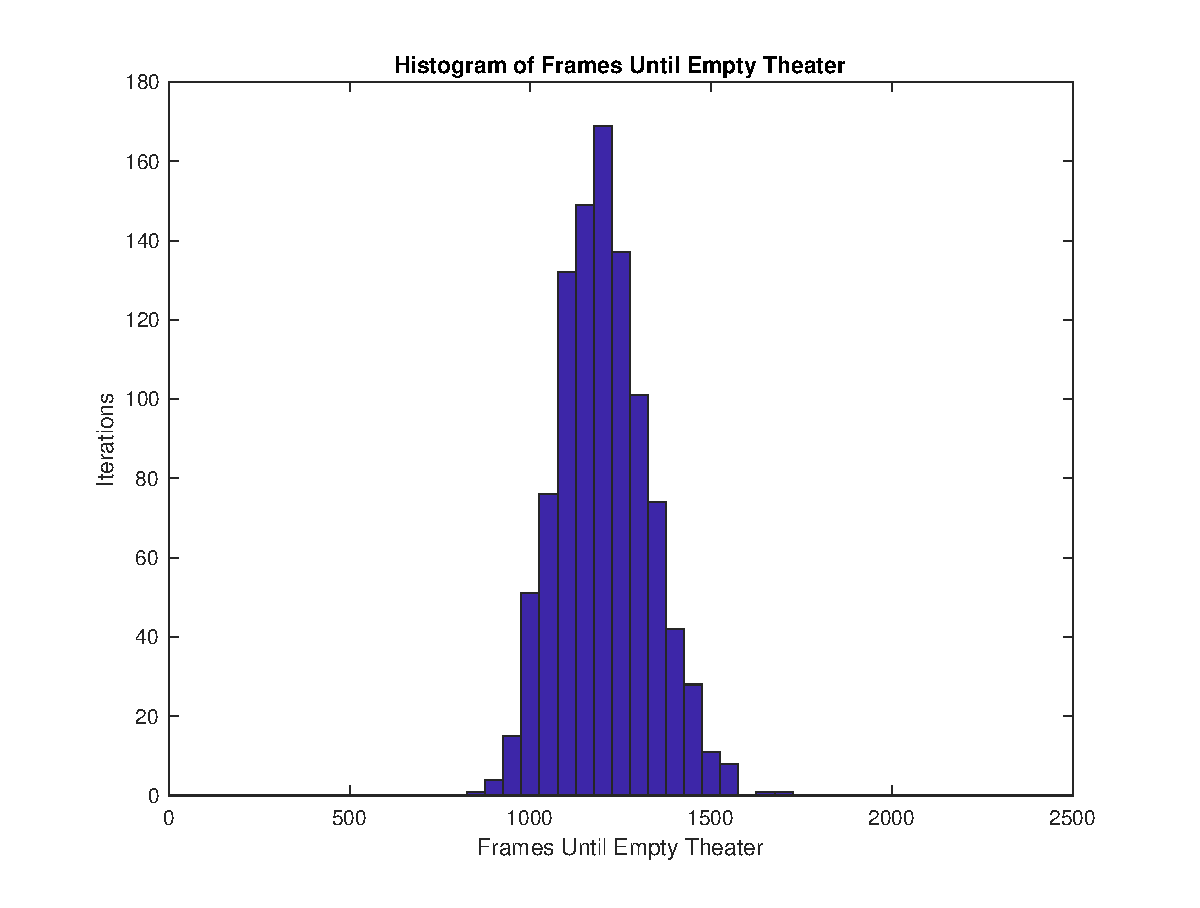
\includegraphics[width=.45\textwidth]{hist_fuet} &
    \includegraphics[width=.45\textwidth]{hist_runtime} 
  \end{tabular}
  \caption{Running the simulation 1000 times, and taking these variables, these histograms were generated.}
\end{figure}

From Figure 3, it is clear that both of these values vary as Log-Normal distributions. Some reasoning as to why might go like this: often, a Log-Normal distribution occurs when there are accruing percentage changes in a system. In this circumstance, this multiplicative effect, in the log of the variable, is additive. If there is an additive effect, drawn from the same distribution, then the Central Limit Theorem applies. This means the log of the variable of interest is a normal, and therefore the variable definitionally varies as a Log-Normal. Given all of the above, the question is really what percentage change is accruing in the simulation. The answer is rather simple: people. As people leave, the simulation will run a percentage faster, there's a percentage lower chance any people are overlapping anything they shouldn't be, etc. The fact that people are removed from the simulation is what makes these variables vary as Log-Normals.

\subsubsection{MLE for the Log-Normal Distribution}

The way the framework is going to get these proven bounds on the value of interest is by fitting the Log-Normal distribution for some number of samples. The next step then is to derive the $\hat{\mu}$ and $\hat{\sigma}^2$ that maximize the log-likelihood function of the Log-Normal distribution.

\begin{equation}
	X_i \sim LogNormal(\mu, \sigma^2)
\end{equation} 

\begin{equation}
	f_{X_i}(x|\mu, \sigma^2) = \frac{1}{x \sqrt{2 \pi \sigma^2}} e^{-\frac{(log(x) - \mu)^2}{2\sigma^2}} 
\end{equation} 

First, the likelihood function, given $X = \{X_1, X_2, \dots X_n\}$, is the product of the probability densities of each $X_i$:

\begin{align}
	L(\mu, \sigma^ | X) &= \prod_{i=1}^{n} f(X_i|\mu, \sigma^2)\\
	&= \prod_{i=1}^{n} \frac{1}{X_i\sqrt{2 \pi \sigma^2}} e^{-\frac{(log(X_i) - \mu)^2}{2\sigma^2}}\\
	&= (2 \pi \sigma^2)^{-\frac{n}{2}} \prod_{i=1}^{n} \frac{1}{X_i} e^{-\frac{(log(X_i) - \mu)^2}{2\sigma^2}}
\end{align}

Next, take the log of the Eq. (8) to get $\mathcal{L}(\mu, \sigma^2 | X)$:
\small
\begin{align}
	\mathcal{L}(\mu, \sigma^2 | X) &= log \Bigg((2 \pi \sigma^2)^{-\frac{n}{2}} \prod_{i=1}^{n} \frac{1}{X_i} e^{-\frac{(log(X_i) - \mu)^2}{2\sigma^2}}\Bigg)\\
	&= -\frac{n}{2}log(2\pi \sigma^2) - \sum_{i=1}^n \Big[ log(X_i) + \frac{(log(X_i) - \mu)^2}{2\sigma^2} \Big]\\
	&= -\frac{n}{2}log(2\pi \sigma^2) - \sum_{i=1}^n \Big[ log(X_i) + \frac{log(X_i)^2 - 2 log(X_i)  \mu + \mu^2}{2\sigma^2}\Big]\\
	&= -\frac{n}{2}log(2\pi \sigma^2) - \sum_{i=1}^n \Big[ log(X_i) + \frac{log(X_i)^2}{2\sigma^2} - \frac{log(X_i)\mu}{\sigma^2} + \frac{\mu^2}{2\sigma^2}\Big]\\
	&= -\frac{n}{2}log(2\pi \sigma^2) - \frac{n\mu^2}{2\sigma^2} - \sum_{i=1}^n \Big[ log(X_i) + \frac{log(X_i)^2}{2\sigma^2} - \frac{log(X_i)\mu}{\sigma^2}\Big]
\end{align}
\normalsize
Now taking the partials, first with respect to $\mu$:

\begin{equation}
	\frac{\partial \mathcal{L}}{\partial \mu} = - \frac{n\mu}{\sigma^2} \sum_{i=1}^n \frac{log(X_i)\mu}{\sigma^2}
\end{equation}

Setting this to zero and solving then:

\begin{align}
	0 &= - \frac{n \hat{\mu}}{\hat{\sigma}^2} + \sum_{i=1}^n \frac{log(X_i)}{\hat{\sigma}^2}\\
	n \hat{\mu} &= \sum_{i=1}^n log(X_i)\\
	\hat{\mu} &= \frac{\sum_{i=1}^n log(X_i)}{n}
\end{align}

Next taking the partial with respect to $\sigma^2$:

\begin{equation}
	\frac{\partial \mathcal{L}}{\partial \sigma^2} = -\frac{n}{2 \sigma^2} - \sum_{i=1}^n \frac{(log(X_i) - \mu)^2}{2 (\sigma^2)^2}
\end{equation}

Setting this to zero and solving then:

\begin{align}
	0 &=  -\frac{n}{2 \hat{\sigma}^2} + \sum_{i=1}^n \frac{(log(X_i) - \hat{\mu})^2}{2 (\hat{\sigma}^2)^2}\\
	\frac{n}{2 \hat{\sigma}^2} &= \sum_{i=1}^n \frac{(log(X_i) - \hat{\mu})^2}{2 (\hat{\sigma}^2)^2}\\
	\hat{\sigma}^2 &= \frac{\sum_{i=1}^n (log(X_i) - \hat{\mu})^2}{n}\\
	\hat{\sigma}^2 &= \frac{\sum_{i=1}^n (log(X_i) - \frac{\sum_{i=1}^n log(X_i)}{n})^2}{n}
\end{align}

So the maximum likelihood estimators for the Log-Normal distribution are:

\begin{align}
    \hat{\mu} &= \frac{\sum_{i=1}^n log(X_i)}{n}\\
	\hat{\sigma}^2 &= \frac{\sum_{i=1}^n (log(X_i) - \frac{\sum_{i=1}^n log(X_i)}{n})^2}{n}
\end{align}

\subsubsection{Minimum Samples for Accurate Log-Normal MLE}

Using the methodology developed by Psutka and Psutka \cite{psutka_psutka_2015} for the normal distribution, lower bounds can be derived for the number of samples for a given certainty of a given confidence of accurate maximum likelihood estimates.  It is relatively easy to adapt their methods to the Log-Normal distribution.

\paragraph{Expected Log-Likelihood}

First we need a way to evaluate the accuracy of a likelihood estimate. The best way to evaluate this accuracy would be to ask: given the true parameters of $\mu$ and $\sigma$, what would the value of the log-likelihood function be? The answer is that it would be the expected log-likelihood function. The expected log-likelihood function is defined as:

\tiny
\begin{align}
	E[\mathcal{L}] &= \lim_{N\rightarrow\infty} \Big( \frac{1}{N} \sum_{i=1}^N \mathcal{L}(\mu, \sigma^2 | X) \Big)\\
	&= \lim_{N\rightarrow\infty} \Bigg( \frac{1}{N} \sum_{i=1}^N \Big( -\frac{n}{2}log(2\pi \sigma^2) - \frac{n\mu^2}{2\sigma^2} - \sum_{i=1}^n \Big[ log(X_i) + \frac{log(X_i)^2}{2\sigma^2} - \frac{log(X_i)\mu}{\sigma^2}\Big] \Big)\Bigg)\\
	&= -\frac{n}{2}log(2\pi \sigma^2) - \frac{n\mu^2}{2\sigma^2} - \lim_{N\rightarrow\infty} \Bigg( \frac{1}{N} \sum_{i=1}^N \Big(\sum_{i=1}^n \Big[ log(X_i) + \frac{log(X_i)^2}{2\sigma^2} - \frac{log(X_i)\mu}{\sigma^2}\Big] \Big)\Bigg)\\
	&= -\frac{n}{2}log(2\pi \sigma^2) - \frac{n\mu^2}{2\sigma^2} - \sum_{i=1}^n \Big[ \lim_{N\rightarrow\infty} \frac{1}{N} \sum_{i=1}^N log(X_i) + \frac{\displaystyle\lim_{N\rightarrow\infty} \frac{1}{N} \sum_{i=1}^N log(X_i)^2}{2\sigma^2} - \frac{\mu \displaystyle\lim_{N\rightarrow\infty} \frac{1}{N} \sum_{i=1}^N log(X_i)}{\sigma^2}\Big]\\
	&= -\frac{n}{2}log(2\pi \sigma^2) - \frac{n\mu^2}{2\sigma^2} - \sum_{i=1}^n \Big[E[log(X_i)] + \frac{E[log(X_i)^2]}{2\sigma^2} - \frac{\mu E[log(X_i)]}{\sigma^2}\Big]
\end{align}
\normalsize

Now with the expected log-likelihood in terms of the expectation of various functions of $X_i$, those expectations must be solved. Starting with the expectation of $log(X_i)$, which is trivial, by the definition of the Log-Normal distribution:

\begin{align}
	log(X_i) &= Y &\sim N(\mu, \sigma^2)\\
	E[log(X_i)] &= E[Y] &= \mu
\end{align}

Similar logic is applicable to the derivation of the expectation of $log(X_i)^2$:

\begin{align}
	Var(Y) &= E[Y^2] - (E[Y])^2\\
	E[Y^2] &= Var(Y) + (E[Y])^2\\
	E[Y^2] &= \sigma^2 + \mu^2\\
	E[log(X_i)^2] &= \sigma^2 + \mu^2
\end{align}

Returning to the expected log-likelihood function:

\small
\begin{align}
	E[\mathcal{L}] &= -\frac{n}{2}log(2\pi \sigma^2) - \frac{n\mu^2}{2\sigma^2} - \sum_{i=1}^n \Big[E[log(X_i)] + \frac{E[log(X_i)^2]}{2\sigma^2} - \frac{\mu E[log(X_i)]}{\sigma^2}\Big]\\
	&= -\frac{n}{2}log(2\pi \sigma^2) - \frac{n\mu^2}{2\sigma^2} - \sum_{i=1}^n \Big[\mu + \frac{\sigma^2 + \mu^2}{2\sigma^2} - \frac{\mu^2}{\sigma^2}\Big]\\
	&= -\frac{n}{2}log(2\pi \sigma^2) - \frac{n\mu^2}{2\sigma^2} - n\mu - \frac{n(\sigma^2 - \mu^2)}{2\sigma^2} + \frac{n\mu^2}{\sigma^2}\\
	&= \frac{n}{2} \Big( \frac{2\mu^2}{\sigma^2} - 2 \mu - log(2\pi\sigma^2) - 1 \Big)
\end{align}
\normalsize

\paragraph{Evaluating Likelihood Accuracy}

Now setting aside for a moment this expected value for log-likelihood, the fraction below will motivate a means for evaluating the accuracy of any estimated $\hat{\mu}$ and $\hat{\sigma}^2$:

\begin{equation}
	\frac{L(\hat{\mu}, \hat{\sigma}^2 | X)}{E[L(\mu, \sigma^2 | X)]} \geq \beta
\end{equation}

This fraction puts the likelihood using the maximum likelihood estimators for the Log-Normal over the expected value of the log-likelihood function, given the true $\mu$ and $\sigma^2$. This is useful, because we now have a fraction that will range between 0 and 1, but that will asymptotically approach 1 as the number of samples $n$ used in the MLE of $\hat{\mu}$ and $\hat{\sigma}^2$ approaches infinity. This means the value $\beta$ is a proxy for estimation accuracy. It is this value we will set to ensure we get within 99\% of the true expected value of the value of interest.

Taking the log of Eq. (40) and rearranging so that we have a less than inequality we have:

\begin{align}
	log\Big(\frac{L(\hat{\mu}, \hat{\sigma}^2 | X)}{E[L(\mu, \sigma^2 | X)]}\Big) &\geq log(\beta)\\
	\mathcal{L}(\hat{\mu}, \hat{\sigma}^2| X) - E[\mathcal{L}(\mu, \sigma^2 | X)] &\geq log(\beta)\\
	E[\mathcal{L}(\mu, \sigma^2 | X)] - \mathcal{L}(\hat{\mu}, \hat{\sigma}^2 | X) &\leq -log(\beta)
\end{align}

\paragraph{Minimum Samples for Accurate MLE}

We will start by defining $\hat{\mu}_i$ and $\hat{\sigma}^2_i$ as the estimates resulting from $i$ random variables in $Y = \{Y_1, Y_2, \dots Y_i\}$. We will also define $Z = \{Z_1, Z_2, \dots Z_k\}$ where $k$ will be a large integer. $Y$ and $Z$ are drawn from the same distribution with parameters $\mu$ and $\sigma^2$. This allows us to define:

\begin{equation}
	i_{\beta}^* = \min_i \{ E[\mathcal{L}(\mu, \sigma^2 | Z)] - \mathcal{L}(\hat{\mu}_i, \hat{\sigma}_i^2 | Z) \leq -log(\beta) \}
\end{equation}

The estimate $i_{\beta}^*$ is by simulating the above procedure. This can be seen in Algorithm 4.

\begin{algorithm}
\caption{This algorithm takes a two large integers, $t$ and $k$, the number of iterations and the size of the test data vector respectively, and an accuracy $\beta$. It returns the minimum number of iterations required to achieve the given accuracy for each of the $t$ simulations.}\label{nsamples}
\begin{algorithmic}[1]
\Procedure{nsamples}{$t, k, \beta$}
\State $\triangleright$ Initialize $i_{\beta}^*$ as a vector of 2's
\State $i_{\beta}^* \gets twos(t,1);$
\For{$i \gets 1:t$}
\State $\triangleright$ Generate two random parameters $\mu$ and $\sigma$
\State $\mu \gets 100*rand$
\State $\sigma \gets rand$
\State $\triangleright$ Draw $k$ samples from the lognormal with parameters $\mu$ and $\sigma$
\State $Z \gets lognrnd(\mu,\sigma,k,1)$
\State $\triangleright$ Repeat the loop until the desired accuracy is reached
\While {$E[\mathcal{L}(\mu, \sigma^2 | Z)] - \mathcal{L}(\hat{\mu}_i, \hat{\sigma}_i^2 | Z) \leq -log(\beta)$}
\State $\triangleright$ Draw $i_{\beta}^*(i)$ samples from the lognormal with parameters $\mu$ and $\sigma$
\State $Y \gets lognrnd(mu,\sigma,i_{\beta}^*(i),1)$
\State $\triangleright$ Estimate $\mu$ and $\sigma$ with $\hat{\mu}$ and $\hat{\sigma}$
\State $\hat{\mu} \gets mean(log(Y))$
\State $\hat{\sigma} \gets \sqrt{var(log(Y))}$
\State $i_{\beta}^*(i) \gets i_{\beta}^*(i) + 1$
\EndWhile
\EndFor
\State \textbf{return} $i_{\beta}^*$
\EndProcedure
\end{algorithmic}
\end{algorithm}

\begin{figure}[htb]
\centering
  \begin{tabular}{@{}cc@{}}
    \includegraphics[width=.45\textwidth]{hist_nsamp} &
    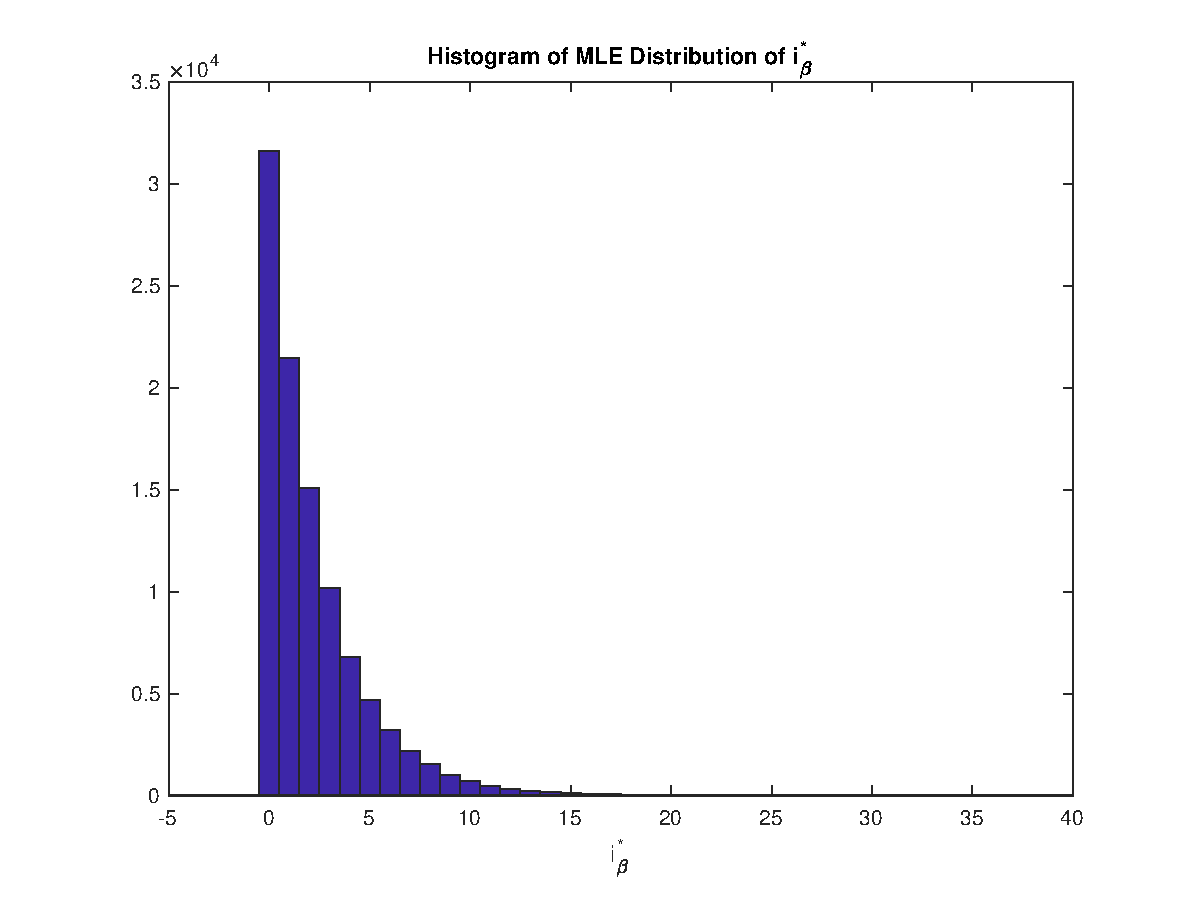
\includegraphics[width=.45\textwidth]{hist_geo} 
  \end{tabular}
  \caption{(Left) This is a histogram of $i_{\beta}^*$; the result of running Algorithm 4 with $t=100000, k=100000, \beta=0.99$. (Right) This is the histogram of 100,000 values drawn from the distribution fit to (Right), using $\hat{p}$.}
\end{figure}

It is clear from Figure 3 that $i_{\beta}^* - 3 \sim Geo(p)$. This also makes sense; there is some probability that the MLE estimate fits the distribution well with only $i$ samples, each iteration we increase the number of samples, running the same experiment, stopping after getting a success. A geometric random variable is defined as the number of experiments before a success, so it makes sense that it would accurately capture this phenomenon. Here too we need to fit this distribution to get the value of $p$. It is therefor necessary to derive the maximum likelihood estimator for the Geometric distribution:

\begin{align}
	L(p | X) &= \prod_{i=1}^n (1-p)^{X_i - 1}p\\
	L(p | X) &= p^n (1-p)^{\sum_{i=1}^n X_i - n}\\
	\mathcal{L}(p | X) &= nlog(p) + (\sum_{i=1}^n X_i - n)log(1-p)\\
	\frac{\partial \mathcal{L}}{\partial p} &= \frac{n}{p} - \frac{\sum_{i=1}^n X_i - n}{1-p}
\end{align}

Setting the partial to zero, and solving for $\hat{p}$:

\begin{align}
	0 &= \frac{n}{\hat{p}} - \frac{\sum_{i=1}^n X_i - n}{1-\hat{p}}\\
	\hat{p} &= \frac{n}{\sum_{i=1}^n X_i}
\end{align}

This estimates the distribution of $i_{\beta}^* - 3$ very well, as is clear from Figure 3, meaning that $\hat{p} = 0.5719$ is a good estimation. Using this value, it is now possible to derive the minimum number of samples that will gauruntee 95\% certainty of being within 99\% of the true expected value:

\begin{align}
	P(i_{\beta} \leq i_{min}) &\geq 0.95\\
	1 - (1-p)^{i_{min} - 1} &\geq 0.95\\
	(1-p)^{i_{min} - 1} &\geq \frac{1}{20}\\
	i_{min} &= log(\frac{1-p}{20} + 1 - p)\\
	&= 4.531
\end{align}

This value is of course 3 short of the actual value, so adding three and rounding up, we have that 8 samples is the minimum required to have 95\% certainty of our MLE estimates being 99\% accurate to the true distribution.

\subsection{Runtime Score}

The minimum simulations for an accurate estimate allows us to write our objective function for runtime. This function is incredibly simple, given a $kT$ and $\sigma_x$, it will hold all other aspects of the simulation constant, and run the simulation 8 times, collecting the runtime of each run, fit a distribution with the maximum likelihood estimators, and return the expected runtime from that distribution.

\subsection{Exit Score}

Similar to the above we can write an objective function for an exit vector. Given a vector of exit positions $e$, the function will hold all other aspects of the simulation constant, and run the simulation 8 times, collecting the number of frames until the theater is empty for each run. It will then fit a distribution with the maximum likelihood estimators, and return the expected runtime from that distribution. The output of this function is the Time To Exit (TTE) described above. 

\section{Optimization}

Everything described up to this point has been independent of the theater being examined. It is at this point that the algorithms described henceforth will have to be run for each theater, to optimize the $n$, $kT$ and $\sigma_x$ for each theater, and then to optimize the exit positions, to get the optimal TTE for a given theater.

The problem is how to actually do these optimizations. Unlike the above problems where it was relatively simple to derive a likelihood function, the objective functions defined in Sections 4.2 and 4.3 seem impossible to differentiate. This means the framework requires a different type of optimization, gradient free optimization.

The framework will utilize two different forms of gradient free optimization, the Nelder-Mead method, and Bayesian Optimization, which will both be explored below.

\subsection{Runtime}

There are several assumptions that underpin the optimization of runtime. First is that the optimal values for $n$, $kT$, and $\sigma_x$ are at least relatively robust if not entirely independent of the exit position. Were this not true, it would be impossible to optimize these runtime variables. The second assumption is that we have a ``reasonable" solution with which to do the optimization. This will likely be a human selected exit vector that does not by any means have to be optimal, but cannot be very bad (there will always be some exit positions where people never leave, or would take so long to escape that it isn't worth the simulation time). This is necessary otherwise it would be similarly impossible to do the runtime optimization. 

\subsubsection{Setting the number of iterations}

The first value to set is $n$, because it will not require any gradient free optimization. It is, at this point, important to draw the distinction between this value, the runtime, and the frames until empty theater. The runtime is the number of real time seconds the algorithm requires to run. The frames until empty theater is the number of accepted moves before all people have evacuated the theater. The number of iterations is the total number of moves attempted, both accepted and rejected. The value $n$ is the maximum number of iterations before the simulation stops. This cutoff is necessary especially when dealing with non-``reasonable" solutions.

How will the framework optimize $n$? It will use the now familiar technique outlined throughout Section 4: 8 runs will be done and the total number of moves required before all people escape will be collected. iterations varies as a Log-Normal, the same as runtime and frames. A distribution will be fit to this data using MLE.

The reason having a good $n$ value is important is because $n$ serves as the cutoff for bad simulations, which are also the most time consuming simulations. So ideally $n$ will be the lowest possible value while cutting short the fewest possible ``reasonable" solutions.

To achieve this the framework sets $n$ to the value for which 95\% of reasonable solutions will have completed, according to the distribution fit above.


\subsubsection{Nelder-Mead}

The Nelder-Mead method attempts to find a global minimum for some real valued function over some number of variables. In this case, it will be minimizing the runtime score function with respect to $kT$ and $\sigma_x$. For higher dimensional problems Nelder-Mead never really converges, but for the simple case of 2 variable optimization assuming a mono-modal function it is a very efficient solution.

This leads to the question of whether the runtime score objective function is mono-modal. Considering the variables independently makes this more clear. 

For $\sigma_x$, the larger the value, the further people can move in a time step, the faster they can conceivably get to the exit. So $\sigma_x$ should be as large as possible, except the bigger $\sigma_x$ is, the higher the chance that people overlap something they shouldn't and the move is rejected. This means $\sigma_x$ likely has an optimum value where the tradeoff between rapid movement and increased move rejection makes sense. 

For $kT$ the tradeoff is more explicitly about tuning the ratio of accepted to not accepted moves based on how ``good" the move is. The closer $kT$ is to zero, the less likely it is to accept any positive change in energy. This means it will reject many more moves, but the moves it accepts are guaranteed to move people towards the exits. Here too there is an obvious tradeoff between two competing factors that scale proportionally, meaning there is a single optimal value.

If $kT$ and $\sigma_x$ both have optimal values then the objective function of these variables will be convex assuming it can be factored in terms of $kT$ and $\sigma_x$. While we cannot prove that the objective function can be factored (in fact it probably cannot be), the effect of changing $kT$ on the optimal value of $\sigma_x$ is experimentally relatively small, meaning the function is very likely convex.

At the highest level, the way Nelder-Mead works is through a simplex, which is a set of $k+1$ points in $k$ dimensions. It is helpful to think of this simplex as a vehicle for exploring the space of the algorithm. There are a set of rules that govern how the simplex can move, and these rules essentially ensure that the simplex will continue to wander to lower points on the function surface while also minimizing it's own area. In this way, the Nelder-Mead method achieves a global minima, without the use of any derivatives. \cite{NeldMead65} 

\begin{algorithm}
\caption{To minimize a function $f(x) \ni x \in \mathbb{R}^n$ Nelder-Mead takes a vector of test points $X=\{X_1,x_2 \dots X_{n+1}\}$, where $f(X)$ will return a vector of evaluations of $f$ for each point in x. This implementation is basically the same as that in the original paper.\cite{NeldMead65}}\label{neld-mead}
\begin{algorithmic}[1]
\Procedure{order}{$X$}
\State $\triangleright$ Reorder x by the value of $f(X_i)$
\State $X \gets X(index_sort(f(X)))$
\If (stop = true)
\State \textbf{return} $X$
\EndIf
\State $\triangleright$ Get the centroid of all points except the point with the highest 
\State $\triangleright$ evaluation of $f(X_i)$, $X_{n+1}$
\State $X_0 \gets centroid(X(1:-1))$
\State \textbf{return} $reflect(X)$
\EndProcedure

\Procedure{reflect}{$X$}
\State $X_r \gets X_0 + \alpha(X_0 - X_{n+1})$
\If {$f(X_1) \leq f(X_r) \leq f(X_n)$}
\State $\triangleright$ If the reflected point is good but not the best, 
\State $\triangleright$ replace the worst point and start again
\State $X_{n+1} \gets X_r$
\State \textbf{return} $order(X)$
\EndIf
\If {$f(X_r) < f(X_1)$}
\State \textbf{return} $expand(X)$
\EndIf
\If {$f(X_n) \leq f(X_r)$}
\State \textbf{return} $contract(X)$
\EndIf
\EndProcedure

\Procedure{expand}{$X$}
\State $X_e \gets X_0 + \gamma(X_r - X_0)$
\If {$f(X_e) < f(X_r)$}
\State $\triangleright$ If the expanded point is better than the reflected point, 
\State $\triangleright$ replace $X_{n+1}$ with the expanded point and start again
\State $X_{n+1} \gets X_e$
\State \textbf{return} $order(X)$
\EndIf
\If {$f(X_r) < f(X_e)$}
\State $\triangleright$ If the expanded point is worse than the reflected point, 
\State $\triangleright$ replace $X_{n+1}$ with the reflected point and start again
\State $X_{n+1} \gets X_r$
\State \textbf{return} $order(X)$
\EndIf
\EndProcedure

\Procedure{contract}{$X$}
\State $X_c \gets X_0 + \rho(X_{n+1} - X_0)$
\If {$f(X_c) < f(X_{n+1})$}
\State $X_{n+1} \gets X_c$
\State \textbf{return} $order(X)$
\EndIf
\If {$f(X_{n+1}) < f(X_c)$}
\State \textbf{return} $shrink(X)$
\EndIf
\EndProcedure

\Procedure{shrink}{$X$}
\State $X \gets X_1 + \sigma(X - X_1)$
\State \textbf{return} $order(X)$
\EndProcedure
\end{algorithmic}
\end{algorithm}

A little more geometric, and less whimsical understanding can be had if we look explicitly at the two dimensional case. In 2D, the algorithm starts with a triangle (3 points) that sits on the 3D surface of the function. The highest point of the triangle is then moved to lower and lower points by pushing the highest point toward the base of the triangle to various degrees (this procedure is detailed more explicitly in Algorithm 5).

The only major question then is when to stop the procedure. The framework uses a relatively basic stopping condition for its implementation of Nelder-Mead; it stops after 400 iterations. It is a rule of thumb to stop after 200 times the number of variables to optimize, so this will ensure a relatively good optimum without spending too much time on the optimization. \cite{lagarias_98} 

After this, with the optimized values for $kT$ and $\sigma_x$ the framework moves on to optimizing the exit position.


\subsection{Exit Position}

For optimizing exit position, the Nelder-Mead algorithm will not work. If we are optimizing exit position for a stadium that holds thousands or tens of thousands then there will be dozens of exits, and Nelder-Mead will simply never converge. Even for a small number of exits, it is very unlikely exit position is a mono-modal surface (consider a simple, symmetrical theater with two exits, the exit score for this function is at least bi-modal as at the optimal positions the exits can be flipped to achieve the same peak at a different input point).

This means the framework must use some other gradient free optimization algorithm, preferably one that requires minimal iterations, as the exit score is expensive to evaluate. This leads us to Bayesian Optimization.

The way Bayesian Optimization works is by treating the objective function as a random function (which exit score actually is). If the objective is a random function, then we can place a prior over the domain of the random function. This prior is designed to capture our belief about the behavior of the function. The function is then evaluated for some number of initial randomly chosen points, and these points are used to update the prior in Bayesian fashion, generating a posterior distribution. This posterior distribution is then used to maximize the acquisition function to select the next point to evaluate.

This is a very broad overview of why Bayesian Optimization is a good technique for this circumstance, and what specific functions were used at each step in the BO algorithm the framework utilizes. It is by no means comprehensive, and uses  the methodology developed by Snoek, Larochelle, and Adams.\cite{NIPS2012_4522}

\subsubsection{Prior Distribution}

The first step to choosing a reasonable prior is understanding the nature of the optimization problem. We have a vector $e$ of magnitude $D = ||e||$, which contains our exits, but what does that mean? We will say that every exit is a real number $e_i$ and that $e_i \in (0,1)$. For this model, it makes sense to compare apples to apples, so we will say the fraction of the perimeter of the theater that can be exits is a fixed value, $\gamma$. We can then divide this fraction by the number of exits, $\frac{\gamma}{D}$, and say that this is the width of every exit. If we then think of our points as the start position of the exits, and the points plus $\frac{\gamma}{D}$ is the end point of the exit. We can then map the interval (0,1) to the perimeter of the theater. Thus we can transform a vector of real values on the interval (0,1) into a set of $D$ exits on the perimeter of the theater. The goal then is to minimize the exit score $f_e(e)$ with respect to the $e$ vector. We can then define $E^D = (0,1)^D$ as the exit space for a given number of exits $D$.

Gaussian processes provide a powerful prior distribution, taking the form $f: E^D \rightarrow \mathbb{R}$. The defining property of a Gaussian process is that any set of $K$ points $\{e_k \in E^D\}_{k=1}^K$ will generate a multivariate Gaussian on $\mathbb{R}^K$. The $k^{th}$ of these points is then $f(e_k)$. The properties of the resulting distribution on the function of interest are defined by two components, the mean function $m: E^D \rightarrow \mathbb{R}$ and the covariance function $m: E^D \times E^D \rightarrow \mathbb{R}$. To avoid losing generality we can set the mean to zero. For the covariance function, we will use the ARD Mat�rn 5/2 kernel.\cite{NIPS2012_4522} 

We have thus defined our function:

\begin{equation}
	f(e) \sim GP(0,k(e,e'))
\end{equation}


\subsubsection{Posterior Distribution}

To generate the posterior distribution we must fit a Gaussian process model to the available data. A Gaussian process model is defined as:

\begin{equation}
	h(e)^T\beta + f(e)
\end{equation} 

Where $h$ and $\beta$ are essentially hyper-parameters used to fit the model. We can then write:

\begin{equation}
	P(y|f(e_i),e_i) \sim N(y_i|h(x)^T\beta + f(x_i), \sigma^2)
\end{equation}

Where the regression is reduced to an optimization problem, how to set the hyper-parameters to ensure the most accurate fit to the data. This leads us back to the Nelder-Mead method, which efficiently seeks the optimal fit.

\subsubsection{Acquisition Function}

Finally we have the acquisition function. This function is what is actually use to select the next point for evaluation. We use the expected improvement aquisition function, as it is ``better behaved than probability of improvement,"\cite{NIPS2012_4522} but doesn't have any parameters of its own, as some other acquisition functions do.

\subsubsection{Stop Criterion}

The only remaining parameter to set for the Bayesian Optimization function is when to stop the optimization process. The framework will proved the best result for a minimum of 30 iterations \cite{bull_2011} of the optimization process, and beyond that the most major constraint is time and computational resources. 

\section{Conclusion}

In conclusion, we will examine a simple theater to understand how the framework could be used in a regulatory setting to determine whether a theater design is acceptably safe, in terms of time to exit and optimal placement of exits.

\begin{figure}
    \centering
    \includegraphics[width=0.75\textwidth]{empty_theater}
    \caption{This shows the simple theater, one with 8 rows each seating three people, with two exits at the back of the theater. It might represent a classroom, or a small lecture hall.}
\end{figure}

The theater shown in Figure 5 contains all the information the framework needs to evaluate the exit position; the dimensions of the theater, the position of all barriers in the theater, and an initial exit position (assumed to be the ``reasonable" exit position necessary for the runtime optimization).

\subsection{Runtime Optimization}

The framework starts by setting the maximum number of iterations for each simulation, $n$, it does this by simulating the initial exit position 8 times, fitting a distribution, and selecting a minimum number of iterations that will mean 95\% of good simulations will complete. For this theater, that $n = 346055$.

\begin{table}
\begin{center}
 \begin{tabular}{||c | c||} 
 \hline
 Pre-optimization & Post-optimization\\ [0.5ex] 
 \hline\hline
 $kT = 0.05, \sigma_x=0.05$ & $kT = 0.0033, \sigma_x=0.04$ \\
 7.78 s & 3.36 s  \\  
 \hline
\end{tabular}
\caption{These are the runtime scores with the initial and optimized values of $kT = 0.05$ and $\sigma_x=0.05$.}
\end{center}
\end{table}

Using this value of $n$, the framework then optimizes runtime by running the simplex algorithm on the runtime score function. The initial simplex is set with $kT = 0.05$ and $\sigma_x=0.05$. These initialization values were determined experimentally to result in good simplex convergence for this problem. The process of optimization takes approximately one hour, and cuts the simulation runtime by 57\%.

\subsection{Exit Position Optimization}

The framework then moves on to optimizing the exit position. For an in depth view of how this process works and how the Bayesian Optimization algorithm explores the space of possible exit positions, please see the attached video.

The final exit position the Bayesian process achieves is visible in Figure 6.

\begin{figure}
    \centering
    \includegraphics[width=0.75\textwidth]{optimial_theater}
    \caption{This is the optimal value of the exit position, given that the terror is at the front center of the theater. It makes sense because it skews to the back, further from where the terror is, but is otherwise basically symmetrical, which it should be as the theater is symmetrical. It also moves the exits in line with the seating rows to alleviate the incredibly bad bunching issues caused by moving the exits to the back of the theater.}
\end{figure}

\subsection{Evaluation of Original Layout}

Given the exit score function and the optimal exit position, we can use a simple fraction to evaluate how good the original exit position and decide whether to allow the building to be constructed. This motivates the fraction:

\begin{equation}
	\frac{TTE_i-TTE_o}{TTE_o} \leq \Delta
\end{equation}

Where $TTE_i$ is the TTE for the initially submitted plan, and $TTE_o$ is the TTE for the optimal solution derived through the Bayesian Optimization. $\Delta$ is the acceptability threshold set by a regulating body. A reasonable $\Delta$ might be 0.50, which would allow economic actors to at most reduce the safety of a theater by 50\% to still be allowed to move forward with the project.

In this case, the $TTE_i = 2730$, and the $TTE_o = 1261$, so the fraction evaluates to 1.165, which seems like an unacceptably high rate of divergence from the optimal case from a public safety perspective. The architects could be given this feedback, along with the optimal exit position, so they could reevaluate their design, and adapt it to be more amenable to keeping people safe.

Thus far we have very explicitly examined the case of exit position, but the beauty of this framework is that it could be extended to adjust everything about the design of the theater, the spacing of the seats, the angle of the rows of seats, the number and spacing of isles, any quantifiable aspect can be tweaked and optimized. 

Obviously, many factors go into the design of buildings and of the seating spaces inside them. But given that we have the ability, now, to assess whether a room is easy to exit in case of danger, and to adjust the room's design to minimize the time to exit, this seems like an easy requirement to include in new buildings, and perhaps a dramatically life-saving one for years into the future.

\printbibliography

















\end{document}